\documentclass[10pt, conference, compsocconf]{IEEEtran}
\usepackage{epsfig,url}
% correct bad hyphenation here
\hyphenation{op-tical net-works semi-conduc-tor}


\begin{document}
%
% paper title
% can use linebreaks \\ within to get better formatting as desired
\title{Socially Aware Single System Images}


% author names and affiliations
% use a multiple column layout for up to two different
% affiliations

\author{\IEEEauthorblockN{Lokesh Mandvekar}
\IEEEauthorblockA{Computer Science\\
University at Buffalo\\
Buffalo NY USA\\
lsm5@buffalo.edu}
\and
\IEEEauthorblockN{Anandatirtha Sathyaraja}
\IEEEauthorblockA{Computer Science\\
University at Buffalo\\
Buffalo NY USA\\
ans25@buffalo.edu}
\and
\IEEEauthorblockN{Chunming Qiao}
\IEEEauthorblockA{Computer Science\\
University at Buffalo\\
Buffalo NY USA\\
qiao@computer.org}
}

% make the title area
\maketitle


\begin{abstract}
Cloud computing enables users to get access to huge amounts 
of computing resources as desired. There are many popular
commercial cloud service providers which provide resources
to users at a price. These providers can not be trusted as
far as privacy of data is concerned. On the other hand,
people do trust their close friends, relatives and other
social contacts, albeit, to varying degrees. This paper
reports the work-in-progress on S3I(Socially Aware
Single System Images) which allows users to form computing
clusters using resources owned by their social contacts.
It tries to utilize the trust found between people in real
life and translate it to provide trustworthy resource
sharing between them.

\end{abstract}

%\begin{IEEEkeywords}
%cluster; single system image; social networking;

%\end{IEEEkeywords}


\section{Introduction}
\label{sec:Introduction}
% no \IEEEPARstart
Single System Image(SSI)\cite{buyya} allows a user to use multiple
standalone computing resources like a unified enhanced machine.
An SSI provides many interesting features like single
entry point, unified processing space, unified memory
and unified i/o space. Applications developed for 
standalone computers can run unmodified on an SSI cluster,
so there is no porting overhead involved. Applications
designed to use multiple processors concurrently,
can utilize all processors present on the cluster
nodes and also make use of the memories on the cluster nodes as
a single contiguous memory.

By making use of social networking tools, users can share
resources such that his/her social contacts can use these
resources along with their own resources to create SSI
clusters. Such a system is an attractive, inexpensive
and viable alternative to the commercially available cloud
technologies. It gives the user control over his/her data
and who it is shared with.

But such sharing of resources also gives rise to many issues
involving privacy assurance, ownership and access
privileges over different system resources. We propose
an incentive based approach that allows users to allocate
the extent of trust to their social contacts, thus
enabling them to allocate privileges based on the extent
of trust on their social contacts. Our work aims to
provide a framework so that any user can share and utilize others'
resources in a fair and trustworthy way.

\subsection{Kerrighed}
Kerrighed\cite{kerrighed} is an SSI operating system based on
Linux\cite{linux}. It makes a cluster of Linux machines look
like a single SMP machine. Kerrighed is implemented as a set
of kernel modules and patches to Linux kernel version 2.6.30.
There are other technologies available for building SSI, like
OpenSSI\cite{openssi}, and some systems like
DragonFlyBSD\cite{dragonflybsd} have SSI creation
as a future goal. Kerrighed is the only software which provides
most of the desirable SSI features.

Kerrighed uses Linux containers\cite{lxc} to provide SSI
functionality. Each nodes runs a single Linux container
(Figure~\ref{fig:kerrighed-arch}) which runs an SSH\cite{openssh}
daemon on port 2222.

% Place figures/kerrighed-arch here
\begin{figure}[htbp]
 \centering
   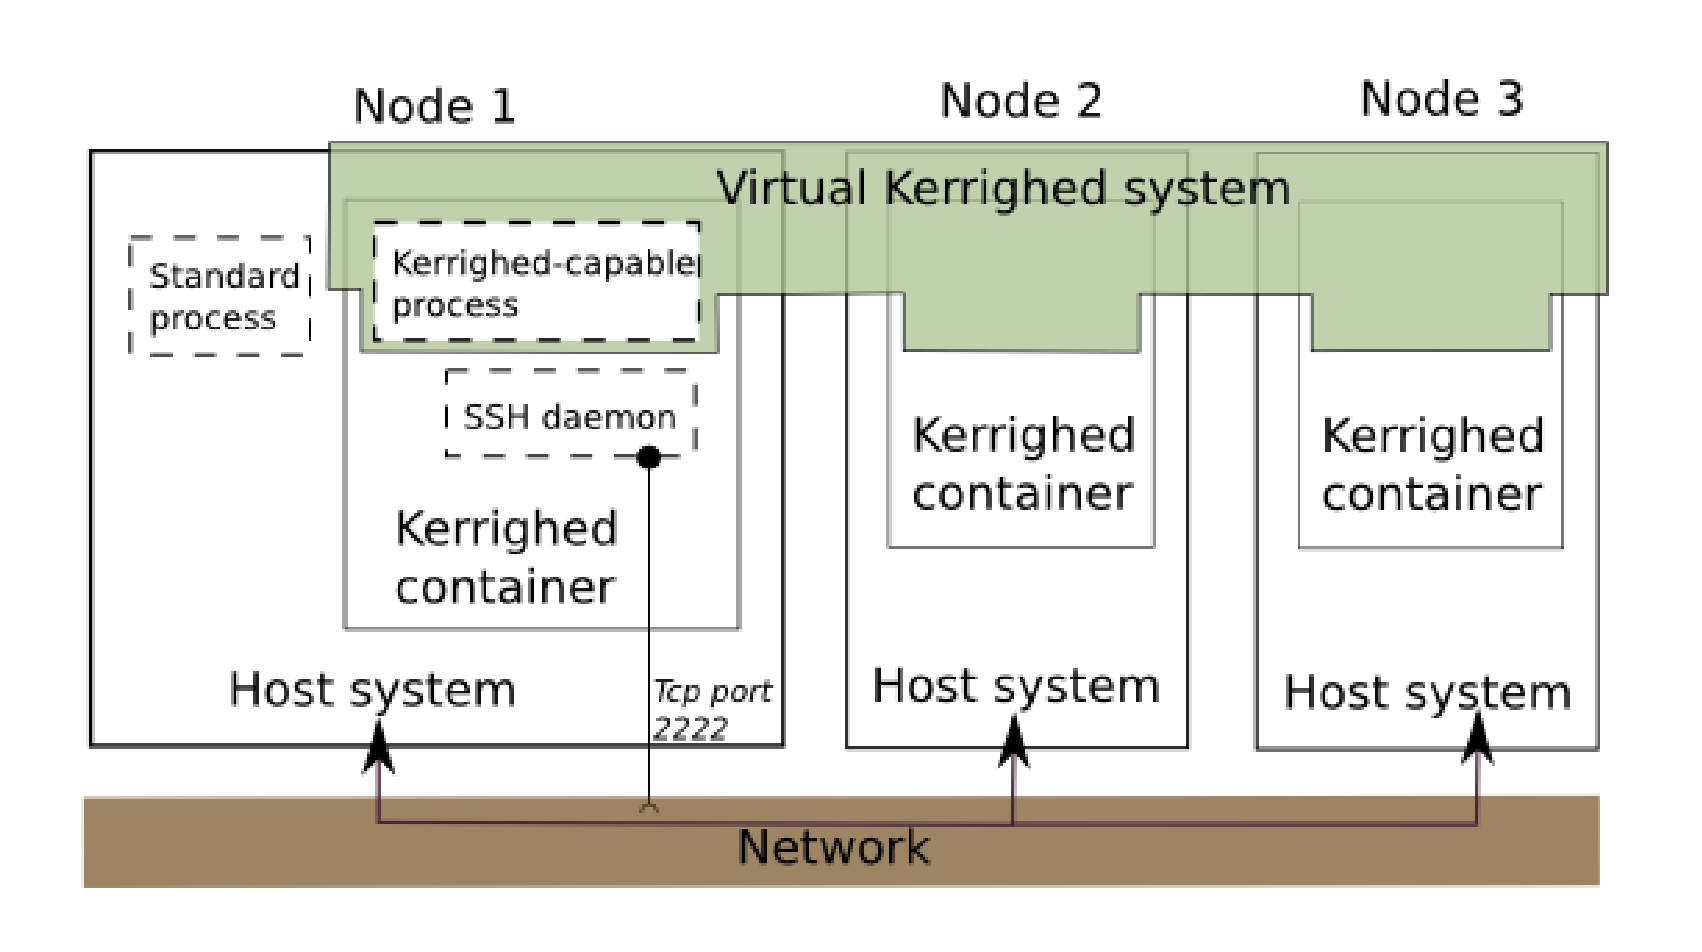
\includegraphics[scale=0.28]{figures/kerrighed-arch}
\caption{Kerrighed architecture}
\label{fig:kerrighed-arch}
\end{figure}

Outside the Linux container, the kernel behaves like an unpatched
kernel and the processor and memory resources visible are only
those physically present on the system (Figure~\ref{fig:kerrighed-local}).

% Place figures/kerrighed-local here
\begin{figure}[htbp]
 \centering
   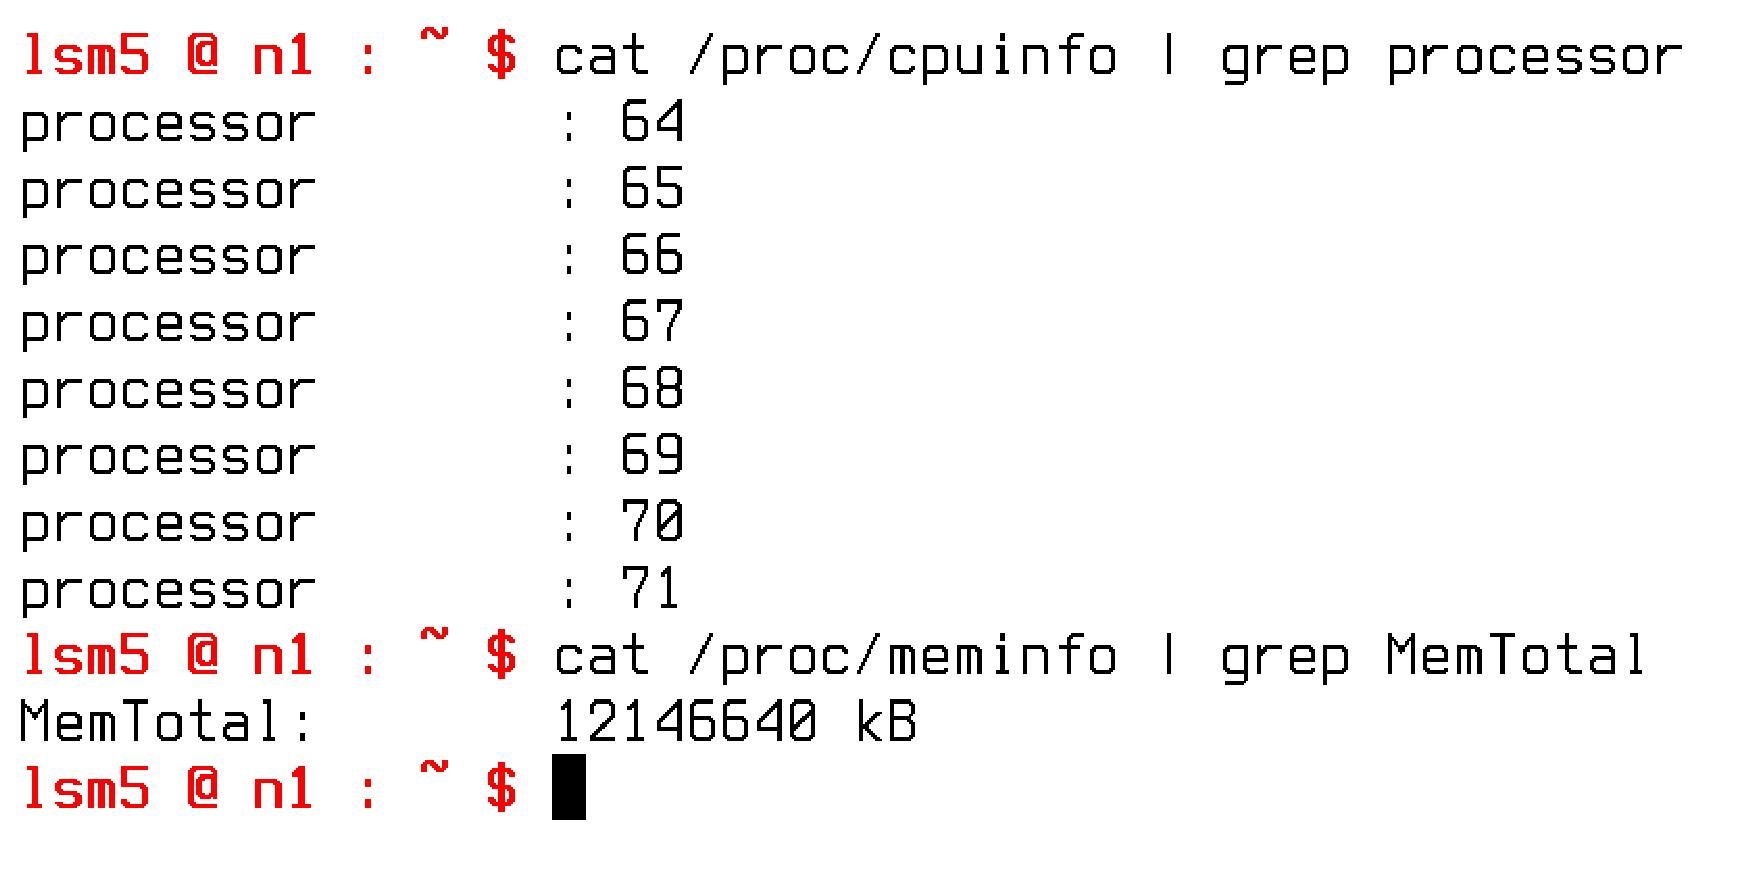
\includegraphics[scale=0.28]{figures/kerrighed-local}
\caption{Resources on the local node}
\label{fig:kerrighed-local}
\end{figure}

All Kerrighed features are accessed by logging into the container.
The nodes present in the cluster are illustrated
(Figure~\ref{fig:kerrighed-nodes}).

% Place figures/kerrighed-nodes here
\begin{figure}[htbp]
 \centering
   
\includegraphics[scale=0.28]{figures/kerrighed-nodes}
\caption{Nodes present in Kerrighed cluster}
\label{fig:kerrighed-nodes}
\end{figure}

Kerrighed presents an aggregated view of the processors on
different nodes in the cluster and presents it in a single
list(Figure~\ref{fig:kerrighed-processors}). Comparing this with
Figure~\ref{fig:kerrighed-local}, we see that the processors on the
other node in the cluster are visible here.

% Place figures/kerrighed-processors here
\begin{figure}[htbp]
 \centering
   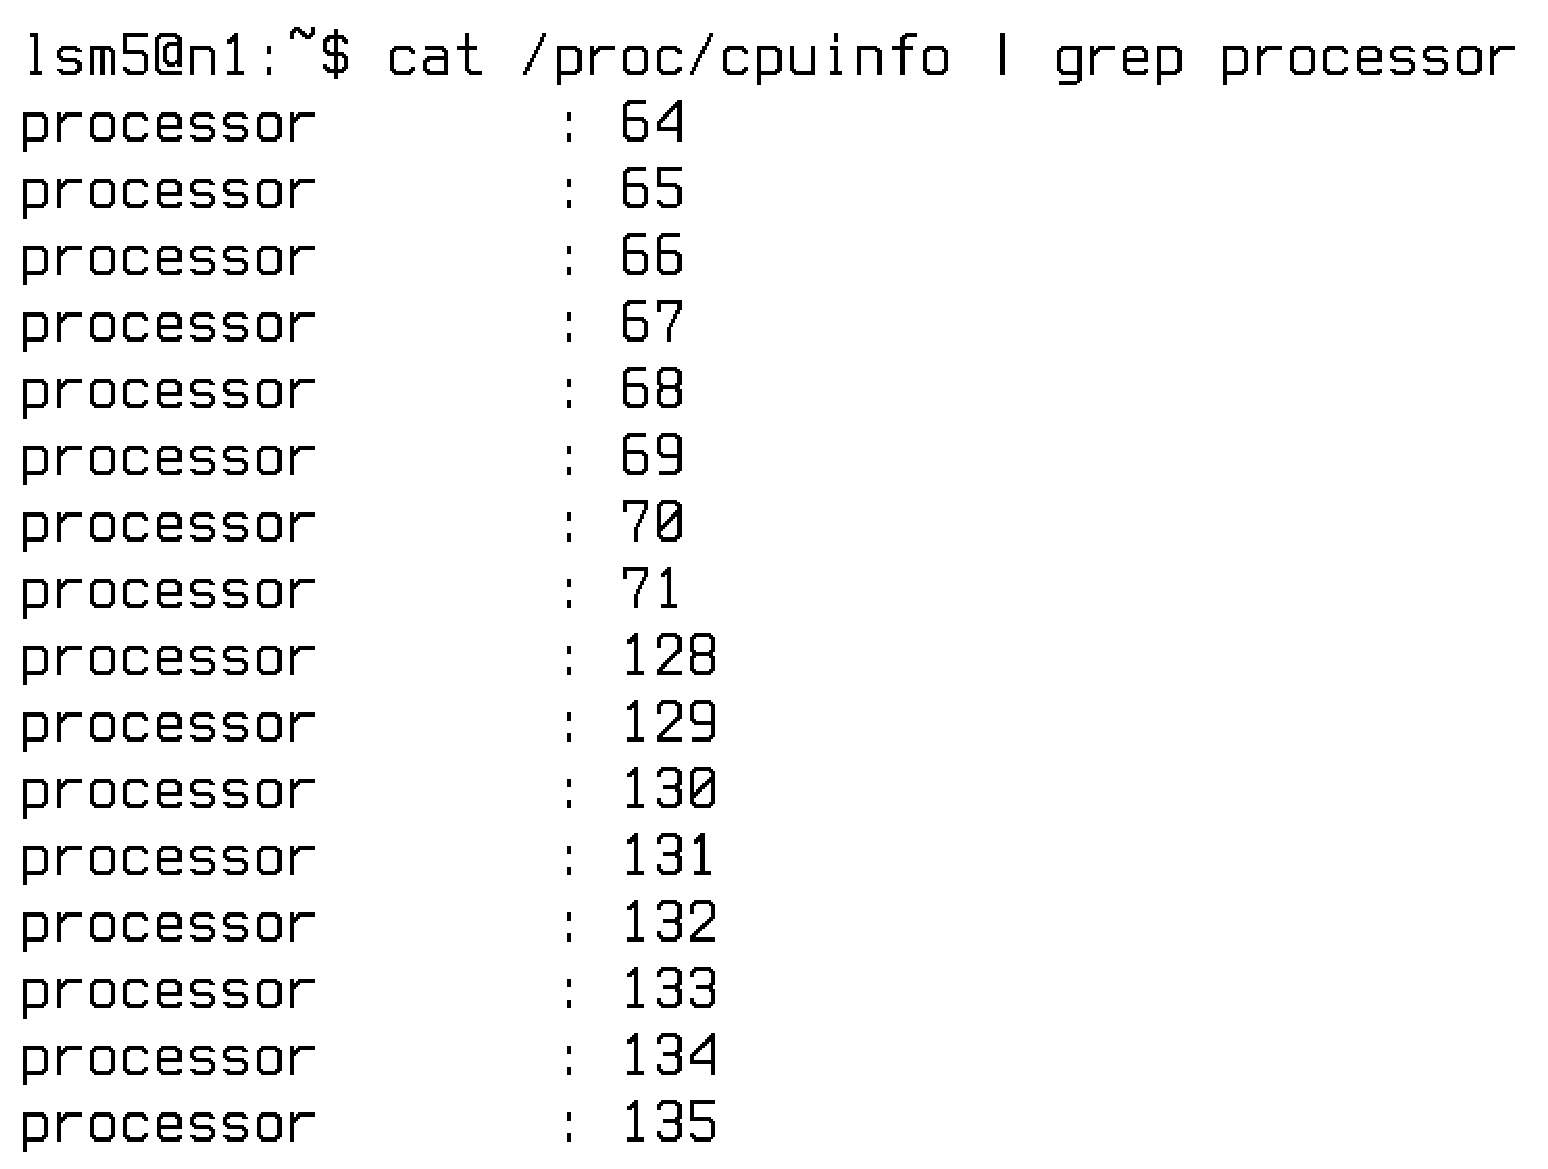
\includegraphics[scale=0.28]{figures/kerrighed-processors}
\caption{Processor cores available in Kerrighed cluster}
\label{fig:kerrighed-processors}
\end{figure}

Kerrighed aggregates the memories of the constituent nodes and presents
it as a single contiguous memory to the user
(Figure~\ref{fig:kerrighed-memory}). In comparison with
Figure~\ref{fig:kerrighed-local}, we see that the other cluster
nodes' memory is added to the memory present on the first node.

% Place figures/kerrighed-memory here
\begin{figure}[htbp]
 \centering
   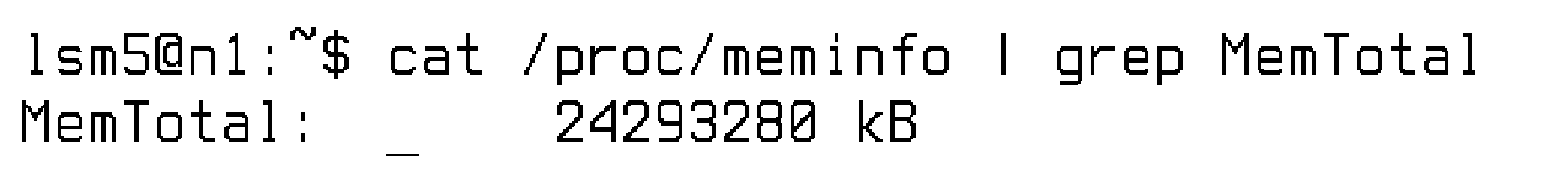
\includegraphics[scale=0.28]{figures/kerrighed-memory}
\caption{Memory available in Kerrighed cluster}
\label{fig:kerrighed-memory}
\end{figure}

The rest of the paper is organized as follows. Section~\ref{sec:Related Work} surveys 
the related work in this area. Section~\ref{sec:Work-in-Progress S3I} reports the current
work-in-progress. It discusses the reputation scheme, and talks
about implementing Kerrighed over wireless networks. Section~\ref{sec:Future Work} outlines
plans for future work. Section~\ref{sec:Geni Usage} describes the utilization of
GENI resources in the project. Section~\ref{sec:Discussion} talks about the expected
publication date of completed work and possible broader impact of the work on GENI.


\section{Related Work}
\label{sec:Related Work}
There are many systems in place which implement user reputation schemes,
based on different aspects like trustworthiness, reliability,
availablility. eBay\cite{ebay} ranks sellers and
customers based on their reliability. StackExchange\cite{stackexchange},
an online Q\&A site, ranks users on the quality of their answers and escalates
their privileges with increasing scores. Online marketplaces like
Bazaar\cite{post}, aim to detect fraud by
malicious participants using user reputation scores. Prior related work
includes a reputation system as a mechanism to provide incentives
to nodes that share resources and provide services to others\cite{gupta}.
The sharing of resources is based on the reputation of the peers. A
credit based system has also been proposed to overcome the
free-rider problem in a P2P network\cite{zhong}.
To the best of our knowledge, no other work aims to provide
trustworthy compute resource sharing between groups of people.


\section{Work-in-Progress S3I}
\label{sec:Work-in-Progress S3I}
S3I extends the idea of SSI, in that, we implement social networking
features wherein users can see a list of physical resources owned by their
social contacts and the access levels allocated to them.
Using this information, the user can choose resources required to build
his/her SSI cluster(Figure~\ref{fig:sassi-screenshot}). We utilize Facebook
APIs\cite{facebook-developer} to provide the social
awareness.


\begin{figure}[htbp]
 \centering
   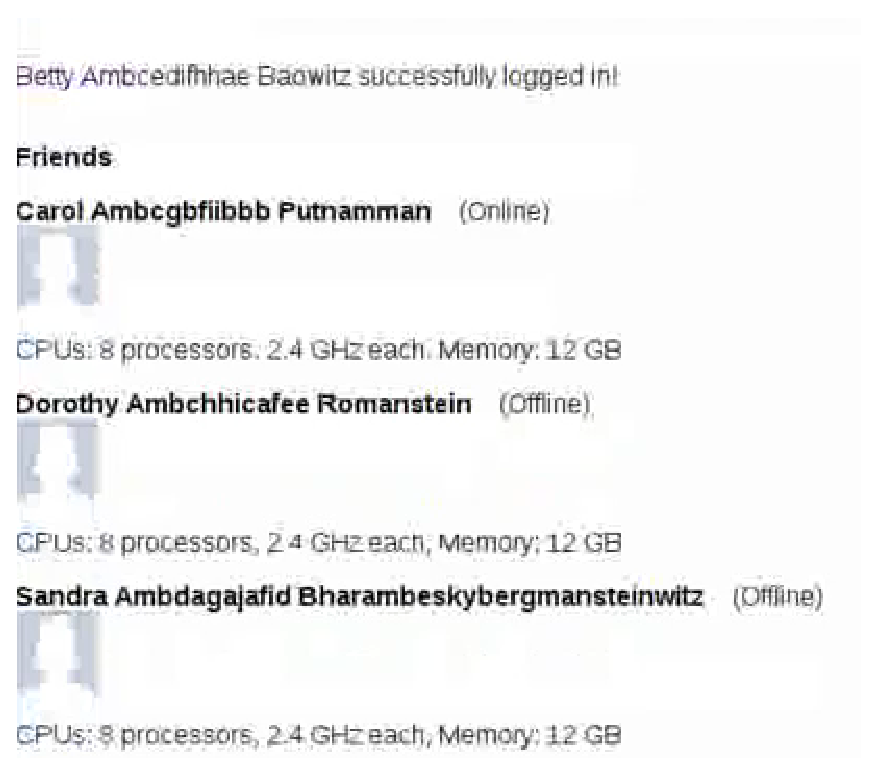
\includegraphics[scale=0.28]{figures/sassi-screenshot}
\caption{Sample Kerrighed interface}
\label{fig:sassi-screenshot}
\end{figure}

\subsection{S3I Workflow}
When a user installs the S3I Facebook\cite{facebook} app,
the user's credentials, and information about his/her compute
resources are collected.
Also, friends of the user, who have also added the app,
are revealed to the user, and the user can selectively add/invite
more people to the application. The user can then select which
resources to use to build/extend his/her cluster.

\subsection{Reputation Scheme}
To an S3I user, there are two broad categories of reputation
scores visible on each friend: Direct (assigned by the 
user himself) and System (the aggregate of scores asigned by
the rest of the users). These are further subdivided into
3 categories: Personal Score, Provider Score, Consumer Score.

\begin{itemize}
\item Direct Personal Score: A user assigned score reflecting
the rapport between a user and his friend.

\item System Personal Score: An aggregate of Direct Personal
Scores assigned to the friend by his/her friends,
reflecting the general personal reputation of the friend.

\item Direct Provider Score: A user assigned score reflecting
the credibility of the friend's resources.

\item System Provider Score: An aggregate of the Direct Provider
Scores assigned by the friend's friends reflecting the
general experience with the friend's resources.

\item Direct Consumer Score: A user assigned score reflecting
the friend’s credibility when consuming the user’s resources.

\item System Consumer Score: An aggregate of the Direct Consumer
Scores assigned by the friend's friends, reflecting the
general credibility of the friend when using others' resources.

\end{itemize}
        
\subsection{Need for Direct and System Scores}
Direct Scores reflect the direct interactions between the
user and his/her friend and are not directly affected by
outside influences. A user will benefit from System Scores
on a friend, since it will give him/her a general idea
of how well the friend interacts with the rest of the world,
and this could serve as an indication of future risks,
benefits, thus possibly influencing the Direct Scores.
A user can directly modify only the direct score for another
user. The system scores will then be modified by the
system itself to account for the updates in the Direct Scores.

\subsection{Kerrighed over Wireless}
We are also evaluating the feasibility of using Kerrighed
over wireless networks, with the end goal of being able
to setup SSI clusters over wireless/adhoc networks.


\section{Future Work}
\label{sec:Future Work}
Our next step after implementing the incentive scheme
is to provide an effective translation of these reputations
to OS-level permissions and access controls. This could
help in automating resource provision with minimum human
intervention allowing the user to establish rules for
setting access controls depending on the reputation.
Also, threats and attacks which could possibly
occur during resource sharing will also be studied and
mitigation schemes implemented.

The propagation of reputation across degrees of separation
and their resultant translation to access controls is also
an interesting aspect. for e.g. Alice and Bob don’t know
each other directly, but Chuck is their mutual friend.
Now if Chuck wants to use Alice's resources, Alice could
estimate Chuck's reputation based on a combination of
Bob's estimated reputation of Chuck and her own
estimated reputation of Bob, and decide whether or
not to give Chuck access to her resources. We are
going to implement automated schemes that would
optimize resource selection based on requirement and
access permissions, to relieve the user from the
intricacies of cluster setup every subsequent time.

SSI setups across wide-area nodes are as yet an unexplored
area. We will study the creation and feasibility of
setting up SSIs using nodes in different sites. Using
SSIs over virtual machines allows a user to partition
his/her resources into discrete sets and each such set
can be potentially shared with different people
simultaneously. The feasibility of such a scheme
will also be studied.

\section{Geni Usage}
\label{sec:Geni Usage}
The ProtoGENI\cite{protogeni} sites in Utah
and Kentucky provide 64-bit Ubuntu\cite{ubuntu}
Linux compute nodes, which are our primary requirement,
because the latest version of Kerrighed is supported
primarily on Debian\cite{debian} based OSes.
We plan to verify the usability of Kerrighed and thus,
S3I, on other 64-bit Linux environments, thus 
extending its usage to other sites, including PlanetLab[18].

\section{Discussion}
\label{sec:Discussion}
The privacy enhancing mechanisms and translation of trusts
to access controls are works in transition, expected to be
completed and submitted for publication by May.

Once the requisite infrastructure is in place,
the creation of such SSI clusters could be extended to
machines on aggregates other than ProtoGENI.
The trust model proposed in this paper, however, is not being
suggested for general purpose usage in GENI at the moment.

\section{Acknowledgment}
\label{sec:Acknowledgment}
We thank the NSF for funding our experiment and GENI
for providing us with infrastructure and support required for the experiment.


\begin{thebibliography}{18}

\bibitem{buyya}
R. Buyya, T. Cortes, H. Jin, Single system image. The International
Journal of High Performance Computing Applications 2001; 15(2):124135.

\bibitem{gupta}
R. Gupta and A. Somani, Game theory as a tool to strategize
as well as predict nodes behavior in peer-to-peer networks. ICPADS 2005.

\bibitem{zhong}
S. Zhong, J. Chen, and Y. Yang, Sprite: A simple, cheatproof,
credit-based system for mobile ad-hoc networks. in INFOCOM 2003.
Twenty-Second Annual Joint Conference of the IEEE Computer
and Communications. IEEE Societies, vol. 3. IEEE, 2003, pp.
1987 - 1997.

\bibitem{post}
A. Post, V. Shah, and A. Mislove, Bazaar: Strengthening user
reputations in online marketplaces. In Proceedings of the
8th USENIX Symposium on Networked Systems Design and
Implementation. USENIX Association, 2011.

\bibitem{kerrighed}
Kerrighed. http://kerrighed.org

\bibitem{linux}
Linux. http://kernel.org

\bibitem{debian}
Debian. http://debian.org

\bibitem{ubuntu}
Ubuntu. http://ubuntu.com

\bibitem{lxc}
Linux containers. http://lxc.sourceforge.net

\bibitem{openssh}
OpenSSH. http://openssh.org

\bibitem{openssi}
OpenSSI. http://openssi.org

\bibitem{dragonflybsd}
DragonFlyBSD. http://dragonflybsd.org

\bibitem{facebook}
Facebook. http://facebook.com

\bibitem{facebook-developer}
Facebook Developers. http://developers.facebook.com

\bibitem{ebay}
eBay. http://ebay.com

\bibitem{stackexchange}
StackExchange http://stackexchange.com

\bibitem{protogeni}
ProtoGENI. http://protogeni.net

\bibitem{planetlab}
PlanetLab. http://planet-lab.org

%\bibitem{kopka}
%H.~Kopka and P.~W. Daly, \emph{A Guide to \LaTeX}, 3rd~ed.\hskip 1em plus
%  0.5em minus 0.4em\relax Harlow, England: Addison-Wesley, 1999.

\end{thebibliography}

\end{document}
